\chapter{Konzeption}
\label{chap:Konzeption}
Dieses Kapitel beschreibt die Resultate und Ergebnisse aus der Konzeptionsphase. Nachfolgend werden auf die verschiedenen Konzeptionsvarianten eingegangen. Dabei werden Überlegungen und Bezüge zur Aufgabenstellung gemacht. Die Varianten werden abschliessend mit einem kurzen Fazit beurteilt. Danach wird mit einem morphologischen Kasten die Komponenten evaluiert für das gewählte Konzept. 

\section{Konzeptionsgrundlage}
\label{sec:Konzeptiongrund}
Als Konzeptionsgrundlage dient das Pflichtenheft, welches im Anhang \ref{Pflichtenheft} einsehbar ist. Wie darin erwähnt, soll das Modul möglichst frei drehend konzipiert werden. Dies ist das ausschlaggebendste Kriterium für die Bauform des Moduls. Da der Velodyne VLP-16, wie in Kapitel \ref{subsec:Velodyne} erläutert, einen begrenzten vertikalen Öffnungswinkel besitzt, wurde bei den folgenden Konzepten die Möglichkeit eines beweglichen Moduls geprüft. Durch eine grösseren Öffnungswinkel kann während der Bewegung der Raum besser ausgemessen werden. Ein weiteres relevantes Kriterium ist die Einsatzmöglichkeit des Modul. Es soll einerseits auf dem Packbot, sowie auch als eigenständiges Produkt funktionieren. Daher sind als Schnittstellen einen Speiseanschluss, welcher 12 Volt Gleichstrom liefert und eine Ethernet RJ45-Anschluss nötig. Nachfolgend sind auf diesen Grundlagen drei Varianten dargelegt.

\section {Variante 1: Plattform}
\label{sec:var1}
Die Variante 1: Plattform ist in der Skizze in Abbildung \ref{fig:plattform} ersichtlich. Bei dieser Konstruktion werden alle elektronischen Komponenten, welche für die Signalverarbeitung und die Energieversorgung nötig sind, in einem rechteckigen Gehäuse im unteren Teil verbaut. Die Interface Box des Velodyne VLP-16 wird auch in diesem Gehäuse untergebracht. Lediglich der Laserscanner VLP-16 befindet sich ausserhalb des Gehäuses auf der Plattform oberhalb des Gehäuses.

\begin{figure}[H]
	\centering
	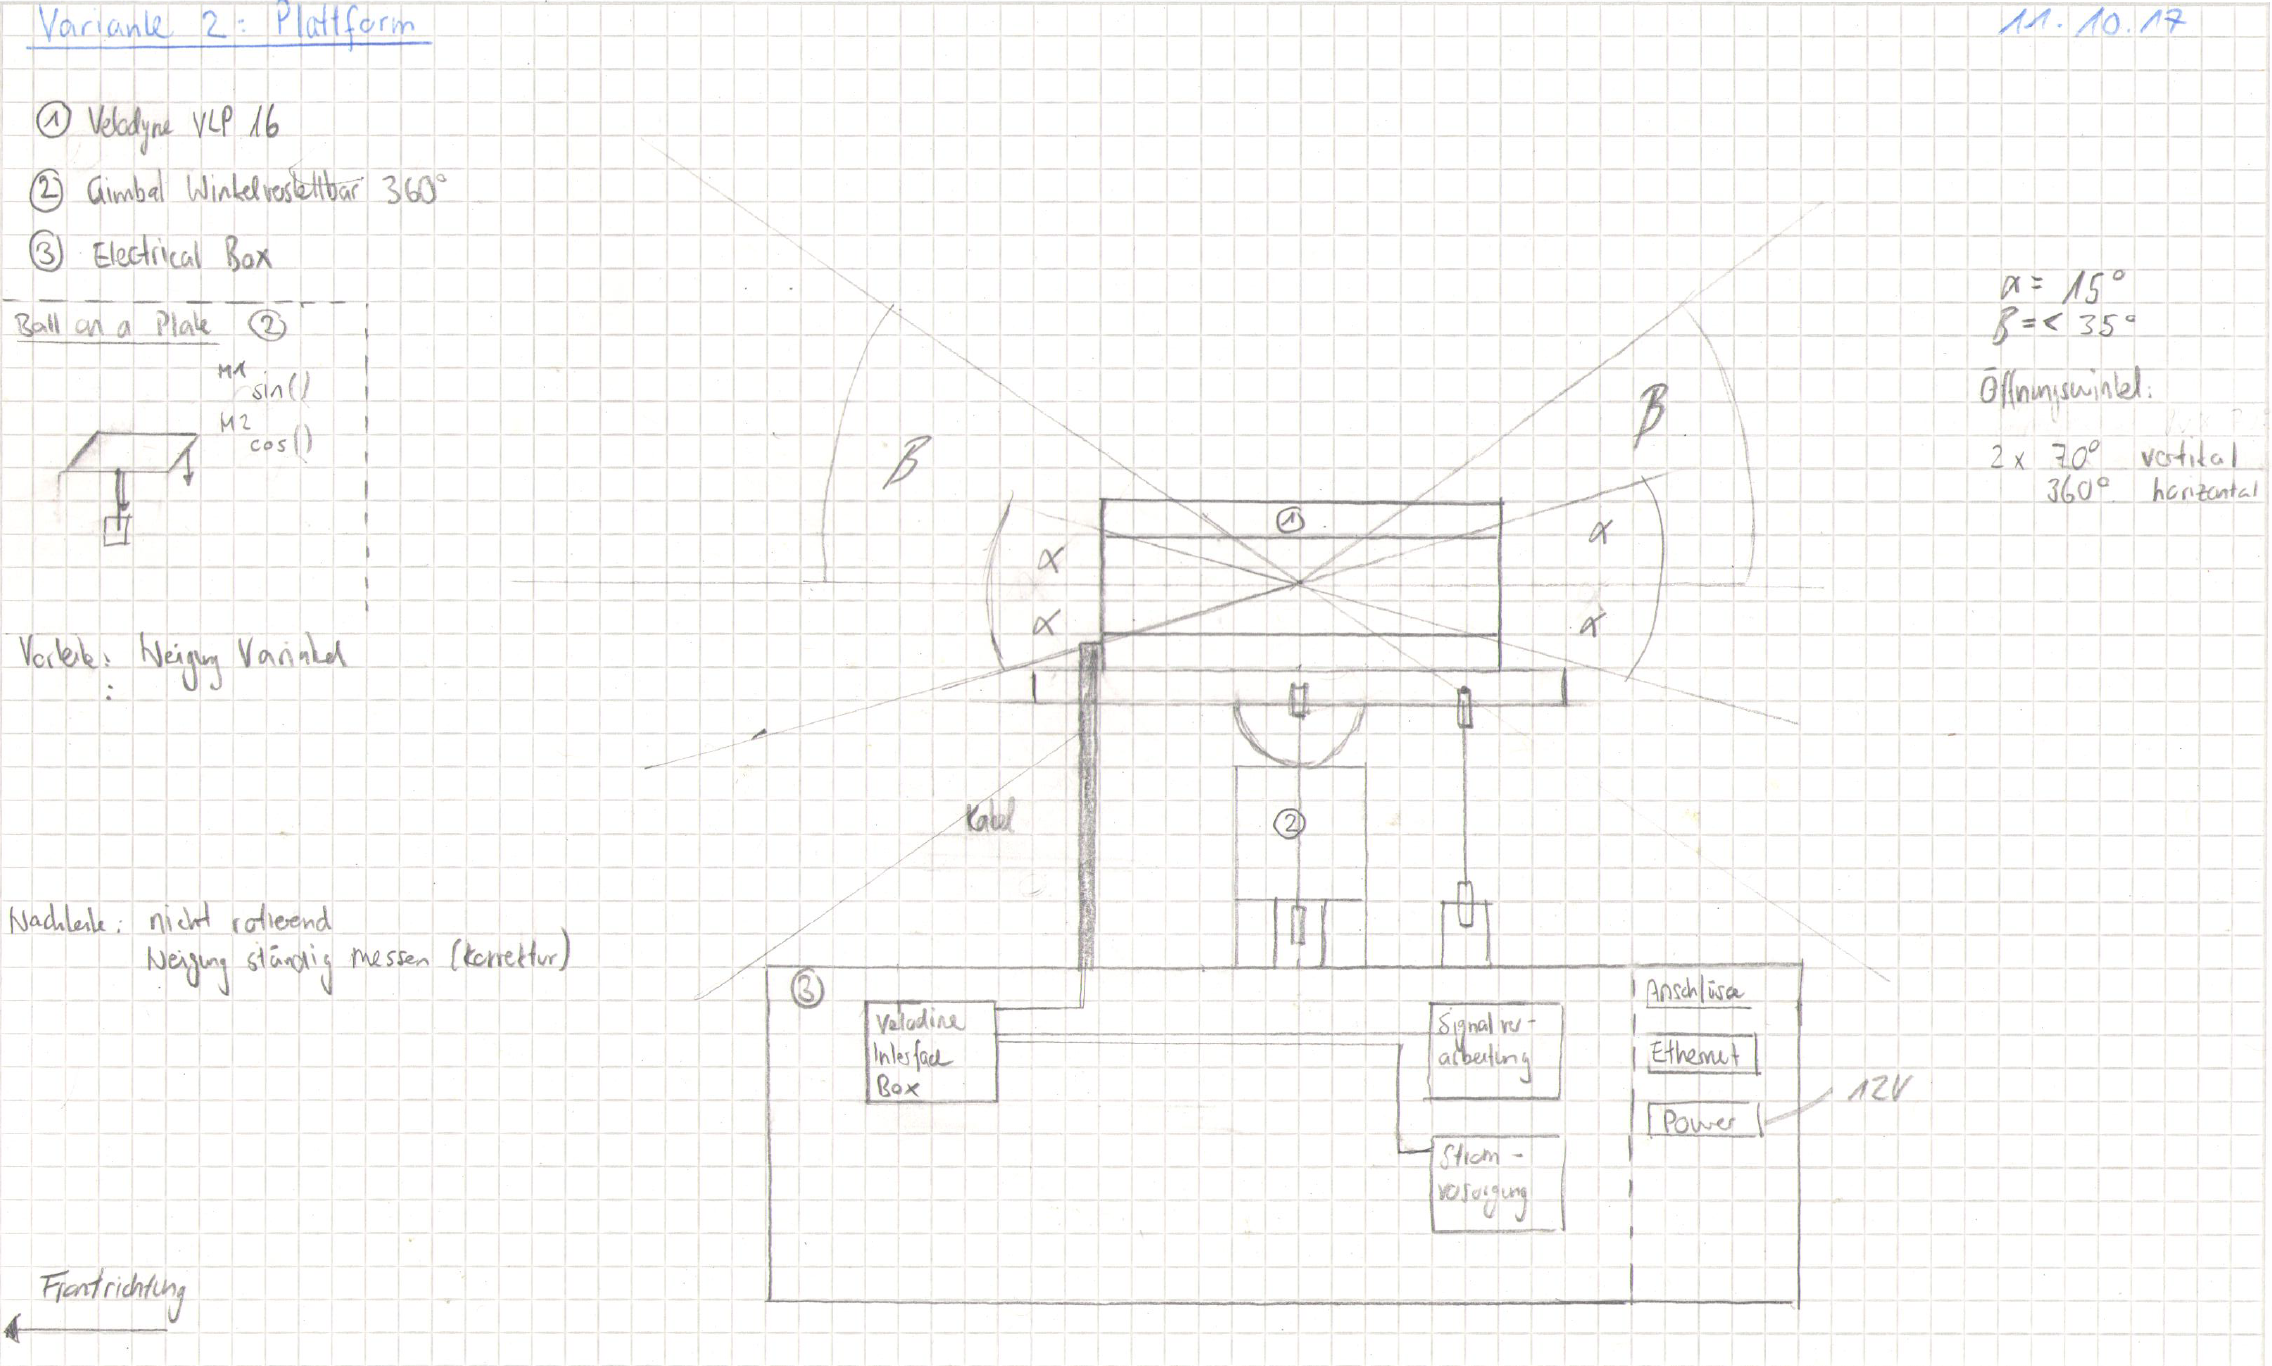
\includegraphics[width=1\textwidth]{resources/skizzev1.PNG}
	\caption[Skizze Variante 1]{Skizze Variante 1}
\label{fig:plattform}
\end{figure} 
	
 Die Eigenheit dieser Konzeption ist die Plattform, auf welcher sich der Velodyne VLP-16 befindet. Der Einsatz dieser Plattform erklärt sich durch ein bekanntes Regelungsexperiment namens "Ball on a Plate". In Abbildung \ref{fig:BalllonaPlateCAD} ist eine CAD-Zeichnung eines solchen Regelungsexperiment dargestellt. Bei "Ball on a Plate" werden zwei Servomotoren, welche je mit einem Gelenk mit einer Seite der Plattform verbunden sind, angesteuert. Indem die Servomotoren mittig auf der Seite mit der rechteckigen Plattform verbunden sind, kann durch Drehen der Servomotoren die Plattform zweiachsig geneigt werden. Im Regelungsexperiment kann durch Zuhilfenahme einer PID-Regelung ein Ball darauf balanciert werden. \cite{ballonaplate}
 
\begin{figure}[H]
	\centering
 	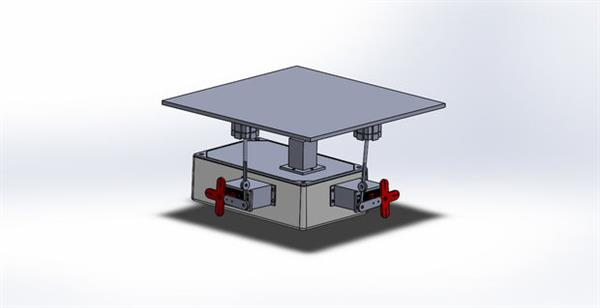
\includegraphics[width=0.8\textwidth]{resources/ballonaplate_cad}
	\caption[Ball on a Plate CAD]{Ball on a Plate CAD {\cite{ballonaplate}}}
	\label{fig:BalllonaPlateCAD}
\end{figure} 

 Diese Überlegungen bieten die Möglichkeit den Laserscanner VLP-16, welcher in der Konzeption auf der Plattform befestigt ist, durch das Ansteuern der Servomotoren in alle Richtungen zu neigen. Somit kann der Öffnungswinkel in jede Richtung vergrößert werden. Die Grenzen liegen dabei im Wesentlichen bei der mechanischen Begrenzung durch die Verbindungsstifte von Platte zu Servomotor.
 
 Hauptproblematik bei dieser Konzeption ist die zusätzlich nötige Sensorik. Durch die Neigung der Plattform kann ohne zusätzliche Sensorik nicht auf die Messausrichtung zurück geschlossen werden. Dies erschwert die Visualisierung der 3D-Laserscanner Messdaten. Die Plattform müsste mittels einer eigenen \ac{IMU}, welche aus Gyrosensor, Accelerometer und Magnetometer besteht, erweitert werden. Zusätzlich ist die Realisierung der Konzeption sehr stark abhängig von den mechanischen Komponenten, da die Verbindungsstifte von Servomotor und Grundplatte die Winkeländerung festlegen.
 

\section {Variante 2: Turm stationär}
\label{sec:var2}
Das zweite Konzept ist eine turmartige Konstruktion, die in Abbildung \ref{fig:skizze_unrotierend} dargestellt ist. Die Idee dazu lieferte das Unterkapitel \ref{subsec:IMM} aus dem Kapitel Informationsbeschaffung. Dabei befindet sich der Velodyne VLP-16 abgesetzt von den elektrischen Komponenten in der Höhe.

\begin{figure}[H]
	\centering
	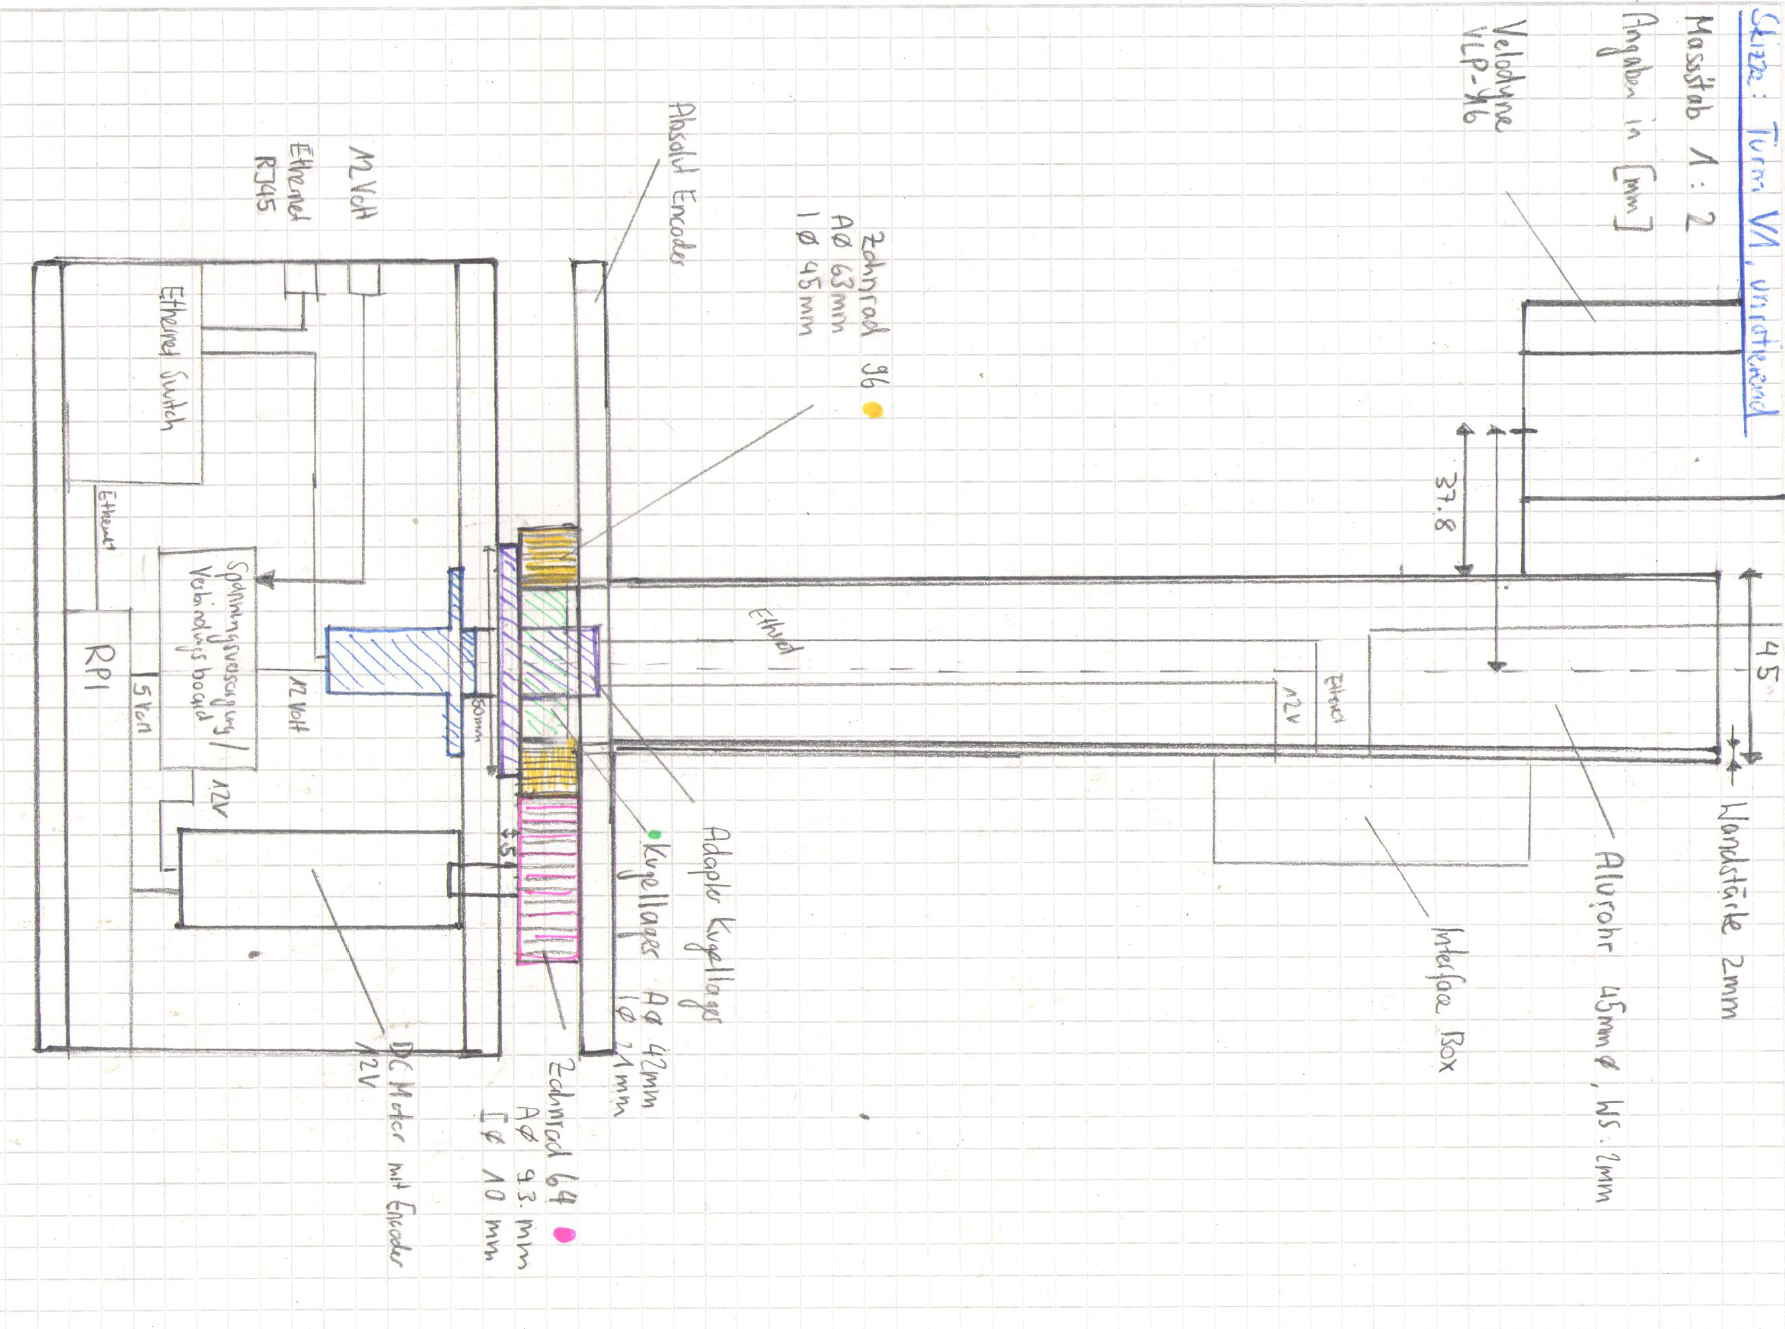
\includegraphics[angle=90,width=0.6\textwidth]{resources/skizze_unrotierend.PNG}
	\caption[Skizze Varainte 2]{Skizze Variante 2 }
	\label{fig:skizze_unrotierend}
\end{figure} 

Eigenheit dieses Konzept ist, dass sich der Turm endlos drehen lässt. Diese Konfiguration verbessert die Problematik des Öffnungswinkel, welche in Unterkapitel \ref{subsec:Velodyne} erläutert ist. Durch die interne Rotation des VLP-16 und den drehenden Turm können Messungen in alle Richtungen getätigt werden. 

In dieser Konfiguration wird der VLP-16 mit einem Motor, der über zwei Zahnräder mit dem Alurohr verbunden ist, gedreht. Der untere Teil des Moduls, in dem sich die Datenverarbeitung befindet, ist stationär. Mittels einem Adapter, an dem ein Kugellager befestigt ist, kann ein möglichst geringe Reibung erzielt werden.

Die gesamte Datenverarbeitung und Ansteuerung wird im stationären Teil getätigt. Die Kabelverbindung des VLP-16 wird über einen Schleifring nach unten geführt. Die Interface Box wird in der Skizze im stationären Teil verbaut. Es ist jedoch auch möglich diese direkt gegenüber des Velodyne zu befestigen. Die Ansteuerung der Motoren und Sensoren, sowie die Datenverarbeitung wird mittels Einplatinencomputer getätigt.

Mittels Nullpunkterkennung und Drehencoder können die aktuellen Positionen an den Einplatinenencoder übermittelt werden.

Nachteil dieser Konfiguration ist, dass es schlecht erweiterbar ist. Da der Schleifring begrenzte Kabeldurchführungen besitzt können keine weiteren Komponenten beim drehenden Teil angeschlossen werden. Ein weiterer Nachteil ist die Problematik, wenn die Rotationsgeschwindigkeit des Turm auf mehrere Umdrehungen pro Minute ansteigt. Es können so fehlerhafte Messresultate beim VLP-16 entstehen.Die Drehgeschwindigkeit des Turms muss verhältnismäßig langsam gegenüber der Drehgeschwindigkeit VLP-16 sein.

Die mechanische Konstruktion ermöglicht auch die Umpositionierung des Velodynes. Wird der Sensor oberhalb des Alurohr befestigt, kann auch die zweite betrachtete Konfiguration des Teams Hector in Unterkapitel \ref{subsec:hector} ausgetestet werden.

\section {Variante 3: Turm rotierend}
\label{sec:var3}
Das dritte Konzept ist wiederum eine Turmartige Konstruktion. Eine Skizze ist in Abbildung \ref{fig:skizze_rotierend} ersichtlich. Es handelt sich hier um eine abgeänderte Version von Variante 2. Dabei befindet sich der Velodyne VLP-16 erneut abgesetzt von den anderen elektrischen Komponenten. Die wesentlichste Änderung liegt darin, dass nun auch die Datenverarbeitung im unteren Teil mitdreht. 
Dies wurde ermöglicht indem alle mechanischen Drehkomponenten und der Motor umgedreht wurden. Somit kann das Problem der Erweiterbarkeit des vorherigen Konzepts gelöst werden. Die gesamte Elektronik und Sensorik dreht nun mit. Lediglich die Schnittstellen Ethernet und 12 Volt Speisung führen über den Schleifring zum Packpot. Für diese Konfiguration wird lediglich zusätzlich ein Alusockel benötigt, welche das Alurohr mit dem Gehäuse verbindet. 

\begin{figure}[H]
	\centering
	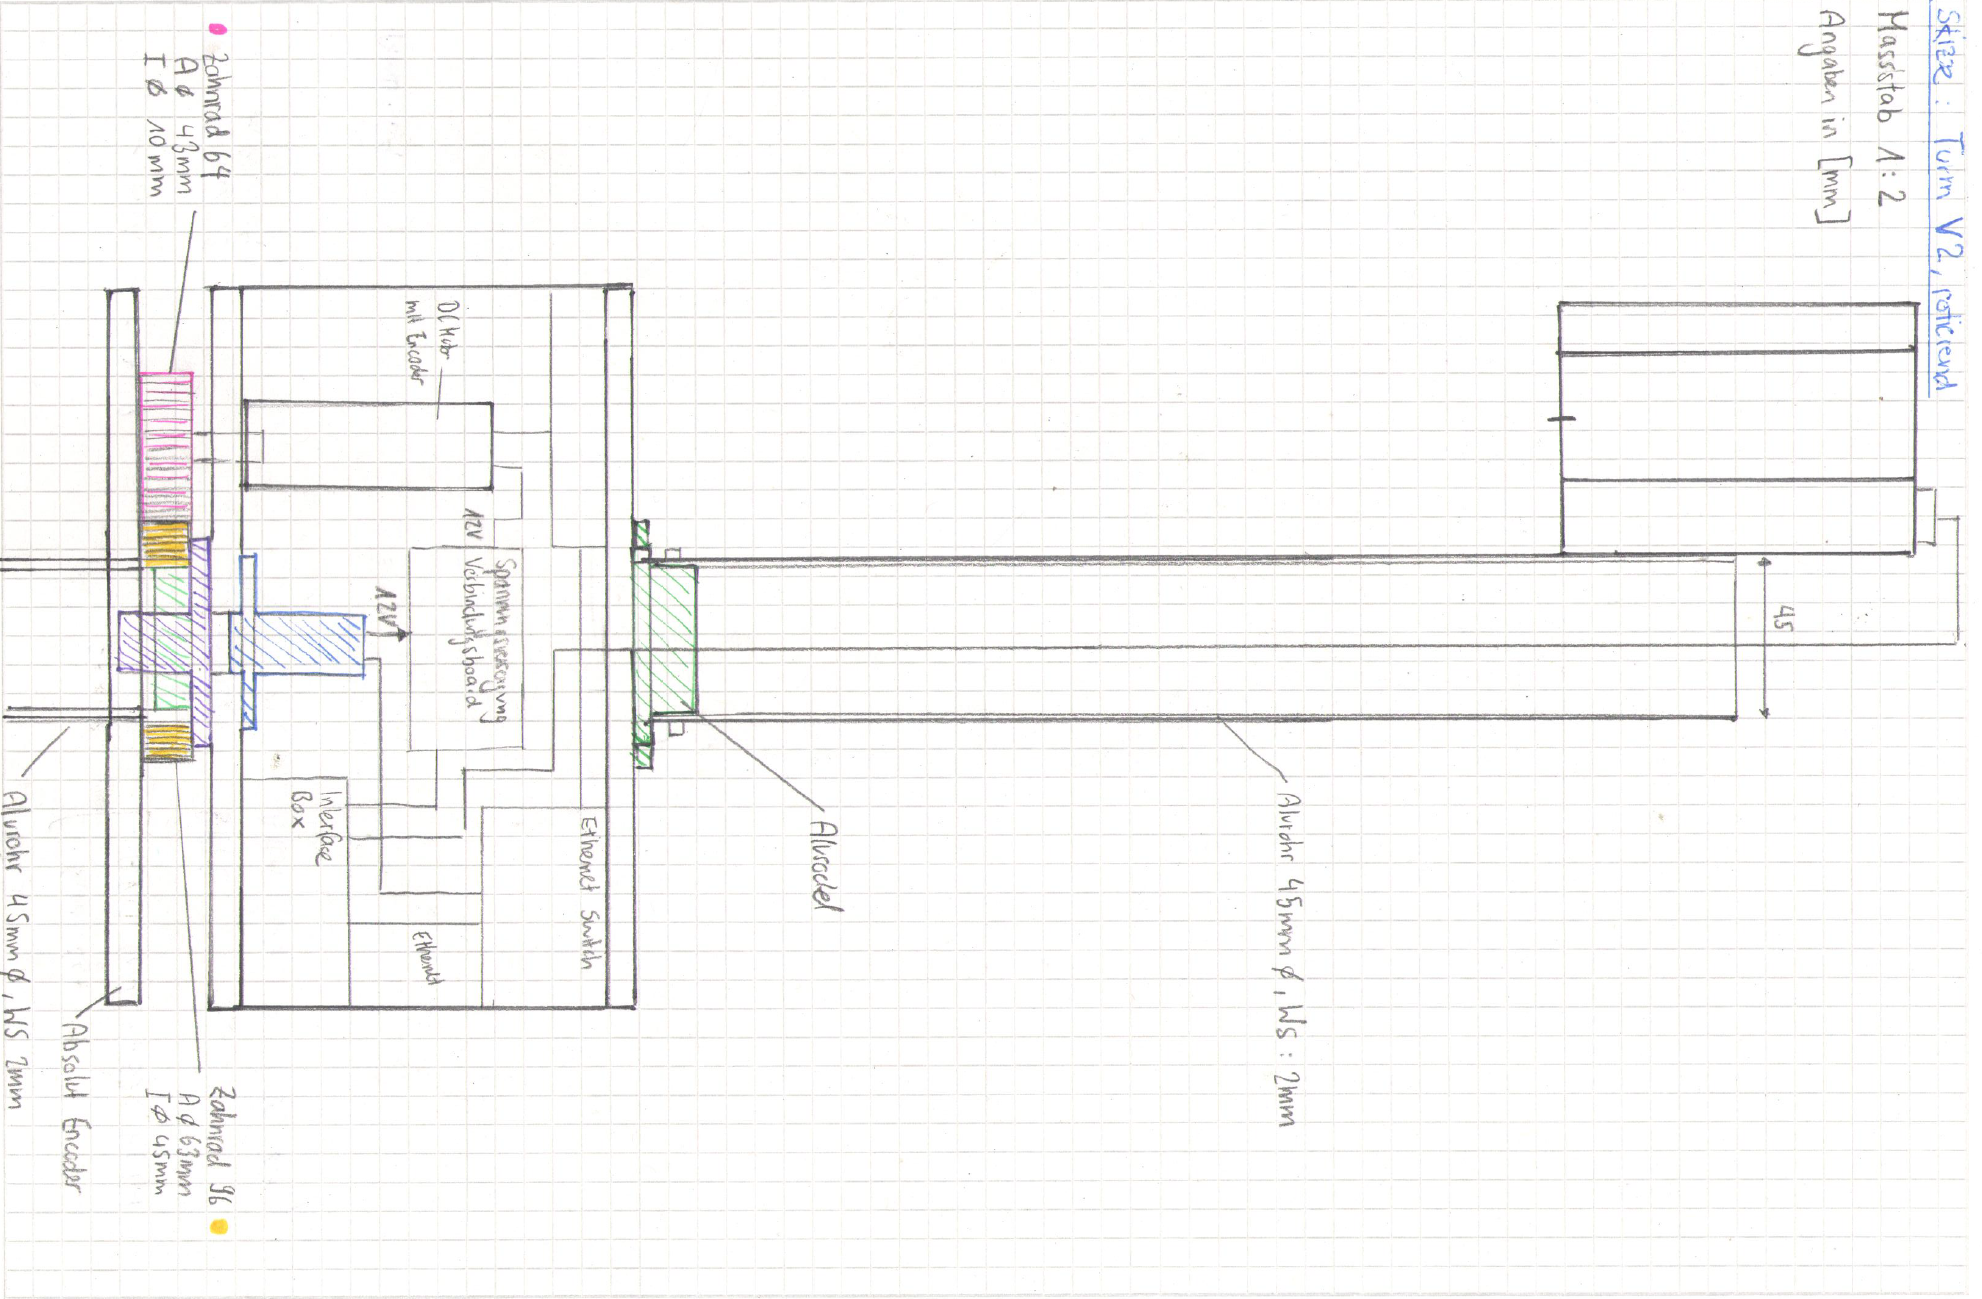
\includegraphics[angle=90,width=0.6\textwidth]{resources/skizze_rotierend.PNG}
	\caption[Skizze Varainte 3]{Skizze Variante 3 }
	\label{fig:skizze_rotierend}
\end{figure} 

Diese Variante bietet jedoch den Nachteil das der Schleifring bedeutend mehr belastet wird. Da alle Komponenten über den Schleifring gespieist werden, müsste eine sorgfältige Berechnung der Strom- und Spannungswerte erfolgen, damit der Schleifring entsprechend ausgelegt wird.

 \section {Konzeptfazit}
 \label{sec:Konzeptfazit}
 
 Da Konzeptvariante 1 bereits frühzeitig verworfen wurde, stehen nur noch die zwei Turm Konzepte gegenüber. Anfänglich wurde die Variante 3 bevorzugt. Während der Zwischenpräsentation vom 8. November 2017 und einer nachträglichen Überarbeitung konnten bedeutende Nachteile der Variante 3 aufgezeigt werden. Einerseits kann die Variante 3 nicht mit einer Bewegungskompensation mittels \ac{IMU} erweitert werden, die für den Einsatz auf dem Packpot nötig ist. Anderseits ist eine bedeutende höheres Drehmoment des Motors nötig, da durch die zusätzliche Elektronik ein bedeutend höheres Gewicht entsteht. Um diese Problem zu verhindern, wurde die Konzipierung der Variante 3 abgebrochen und die Variante 2 ausgewählt. Da die mechanischen Komponenten von Variante 2 und 3 sich kaum unterscheiden, mussten keine groben Zeitverluste hingenommen werden.
 
\section {Evaluation der Komponenten}
\label{sec:ausgewählteKomponenten}
Dieses Kapitel beschreibt die evaluierten Komponenten für die verschieden Teilfunktionen. Die Teilfunktionen wurden bereits im  Kapitel \ref{Informationsbeschaffung} Informationsbeschaffung unterteilt. Für die Entfernungsmessung ist der Velodye VLP-16 vorgegeben. Als Software wurde Ubuntu LTS 16.04 mit ROS Kinetic Kame gewählt. Die Gründe dazu wurden bereits im Unterkapitel \ref{sec:Software} erläutert. Die weiteren Teilfunktionen werden im nachfolgenden morphologischen Kasten gegenübergestellt und danach ausgewählt.

\begin{table}[H]
	\centering
	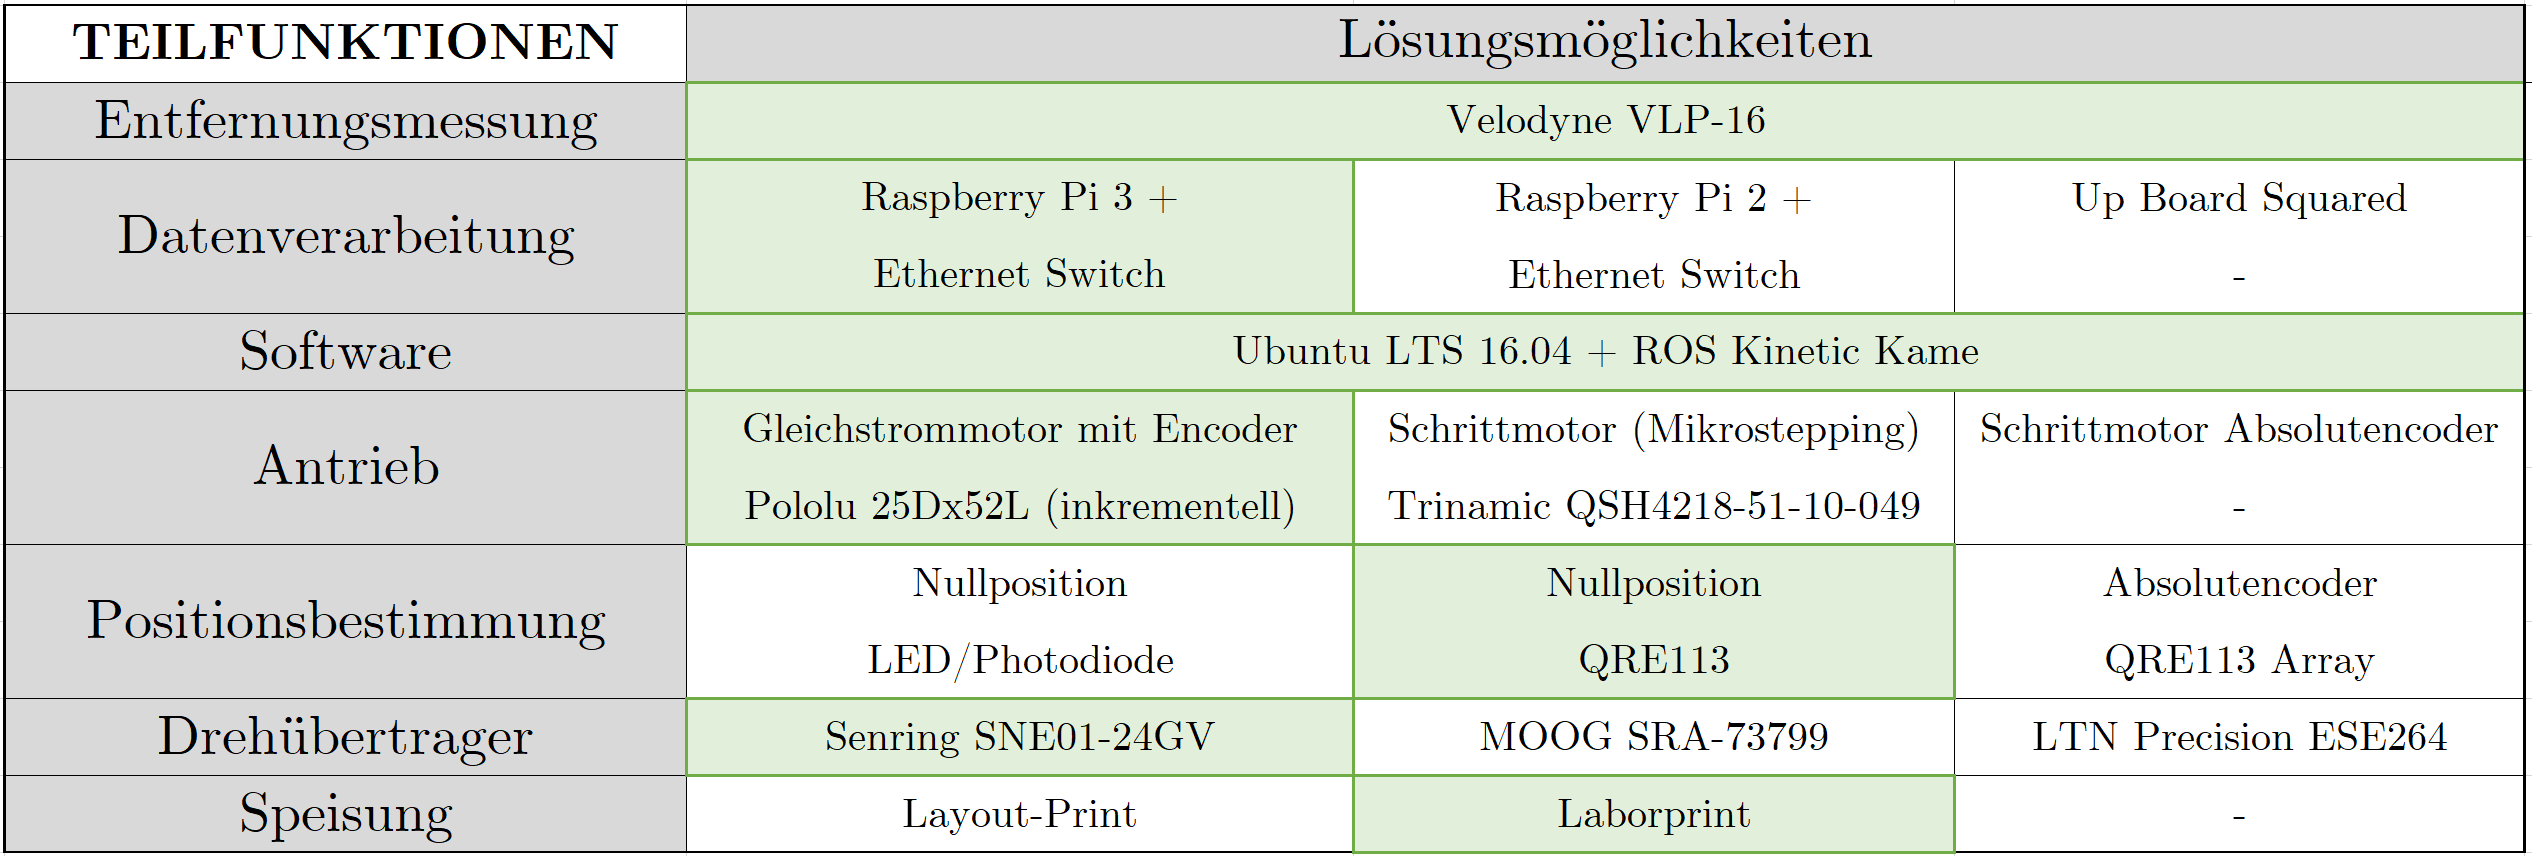
\includegraphics[,width=1\textwidth]{resources/morph.PNG}
	\caption[Morphologischer Kasten]{Morphologischer Kasten}
	\label{fig:morph}
\end{table} 


\subsection{Datenverarbeitung: Raspberry Pi 3}
Im Unterkapitel \ref{sec:Datenverarbeitung} wurden bereits diverse Einplatinencomputer betrachtet und bewertet. Für die Konzeption wurde aus Performancegründen das Raspberry Pi 3 dem Raspberry 2 vorgezogen.  Da das Raspberry Pi 3 nur einen Ethernetanschluss zur Verfügung stellt, wurde der Ethernet Switch DGS-105 von Netgear, welcher bereits im Unterkapitel \ref{subsec:Ethernetswitch} erwähnt wurde hinzugefügt. Dieser Ethernet Switch kann direkt über die verfügbare Speisung von 12 Volt angeschlossen werden. Somit werden alle Datenschnittstellen ermöglicht.  

\subsection{Antrieb: Pololu 25Dx56L}
\label{subsec:pololu}
Schrittmotoren mit Absolutencoder wurden aus Kostengründen in der Evaluation ausgeschlossen. Reine Schrittmotoren sind für die Aufgabenstellung ebenfalls geeignet. Lediglich die Schrittverluste können einen integrierenden Fehler verursachen. Daher wurde für die Aufgabenstellung ein Gleichstrommotor gewählt. Der Pololu 25Dx52 ist ein kompakter 12 Volt Gleichstrommotor mit integriertem 48 \ac{CPR} Encoder. 
D.h. es werden pro Umdrehung 48 Zustände evaluiert, wenn die zwei vorhandenen Hallsensoren verwendet werden. Durch die interne Übersetzung von 46.85:1 ergeben sich 2248.86 CPR. Daraus ergibt sich somit die folgende Auflösung $\frac{360^\circ}{2248.86}$ = 0.160081$^\circ$. 

In einem Messaufbau wurde der Motor angesteuert und ausgetestet. Die zwei Hallsensoren werden über 5 Volt gespeist und über zwei GPIOs auf die die fallenden und Steigende Flanke getriggert. In einer Callback Funktion werden diese Flanken gezählt und über das Verhältnis der aktuelle Winkel eruiert. Die maximale Umdrehungszahl des Motors ist 110 RPM. Durch das lineare Verhalten eines Gleichstrommotors kann durch den Tastgrad eines \ac{PWM} die Umdrehungsgeschwindigkeit mit einem Motorentreiber eingestellt werden. 

\subsection{Positionsbestimmung: Fairchild QR1113}
\label{subsec:QR1113}
Da die inkrementelle Winkeländerung mittels dem Pololu 24Dx56 eruiert werden kann, benötigt es für die Positionsbestimmung lediglich einen definierten Nullpunkt. Der Absolutencoder mit einem QRE 1113 Array fällt für diese Funktion aus. Um eine Auflösung wie im vorherigen Kapitel zu erreichen benötigte es 11 dieser Sensoren. (2$^{11}$ Zustände = 2048). Einerseits werden dazu viele GPIOs benötigt und anderseits ergibt sich durch den Mindestabstand von 4mm zwischen den Sensoren eine grosse Dimension des Drehencoders. Die Dimension enstprich einem Hohlzylinder mit Außendurchmesser 10 cm.
In einem Messversuch wurde mit einem \ac{KO} das Verhalten der LED/Photodiode-Variante und eines einzelnen QRE 1113 ausgetestet. Dabei konnte festgestellt werden, dass mit dem QRE1113 eine bessere Trennschärfe erreicht wird. Dieser Sensor kann bei einem Abstand von 2-3mm von der Oberfläche eine praktisch binäre schwarz/weiss Detektion eruieren. Daher wurde die Variante der Nullposition mit dem Fairchild QR1113 evaluiert.

\subsection{Drehübertager: Senring SNE01-24GV}
\label{subsec:SNE01}
Wie bereits in Unterkapitel \ref{subsec:Schleifring} erläutert ist die Auswahl von Ethernet-Schleifringen bisher noch klein. Es wurde der Senring SNE01-24GV für die Aufgabenstellung evaluiert. Dieser Schleifring ist einerseits mit 120 Fr. der kostengünstigste Schleifring und bietet die erforderlichen Übertagungsmöglichkeiten von Ethernet. Der Schleifring MOOG SRA-73979 und LTN Precision ESE264 sind mit 435 Fr. bzw. 610 Fr. bedeutend teurer. Zusätzlich besitzt der evaluierte Schleifring acht weitere Kabeldurchführungen, von denen zwei Kabel mit 5 Ampere und sechs Kabel mit 2 Ampere belastet werden können.\cite{senring}

\section{Zwischenfazit}
\label{ZwischenfazitKonz}
Die evaluierten Komponenten wurden in einigen Messversuchen ausgetestet und für die Aufgabenstellung als geignet beurteilt. Durch die Sensorkombination kann mit enstsprechender Logik die aktuelle Position ermittelt. Dies ist das wichtigste Kriterium für eine erfolgreiche Softwareimplementation. Die Dimension des Prototypen sind grösstenteils durch die evaluierten Komponenten gegeben. Einzige Verbesserung des Konzepts ist die Lage des Velodyne VLP-16. Wird dieser im Drehpunkt befestigt kann die Differenz zur Drehachse vernachlässigt und somit ein Messfehler kompensiert werden.
\todo{Erklärung weshalb Aufwand für mechanik gerechtfertigt} 



